\documentclass{standalone}
\usepackage{tikz}
\usepackage{ctex,siunitx}
\setCJKmainfont{Noto Serif CJK SC}
\usepackage{tkz-euclide}
\usepackage{amsmath}
\usetikzlibrary{patterns, calc,3d}
\usetikzlibrary {decorations.pathmorphing,decorations.pathreplacing,decorations.shapes}
\tikzset{label style/.append style={font=\small}}
\begin{document}
\small
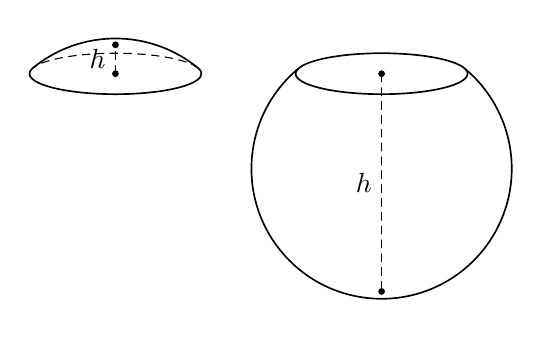
\begin{tikzpicture}[>=latex,scale=0.26]
  \begin{scope}
    \tkzDefPoints{0/0/O,0/6.37/A,0/8.75/H,0/6.05/N,0/-6/N'}
    \tkzDefMidPoint(O,H)\tkzGetPoint{O'}
    \tkzInterCC(O',O)(O,A)\tkzGetPoints{T}{T'}
    \tkzDefPointBy[projection=onto O--H](T)\tkzGetPoint{P}
    \tkzDrawPoints[fill=black](P,N')
    \tkzDrawSegment[densely dashed](P,N')
    \tkzLabelLine[pos=0.5,left](P,N'){$h$}
    \draw[draw=none](P)--++({4.2*cos(15)},{sin(15)}) coordinate(Q);
    \draw[draw=none](P)--++({4.2*cos(165)},{sin(165)}) coordinate(Q');
    \tkzDrawArc[semithick,black](O,Q')(Q)
    \draw[semithick](P)ellipse(4.2 and 1.0);
  \end{scope} 
  \begin{scope}[xshift=-13cm]
    \tkzDefPoints{0/0/O,0/6.37/A,0/8.75/H,0/6.05/N,0/-6/N'}
    \tkzDefMidPoint(O,H)\tkzGetPoint{O'}
    \tkzInterCC(O',O)(O,A)\tkzGetPoints{T}{T'}
    \tkzDefPointBy[projection=onto O--H](T)\tkzGetPoint{P}
    \tkzDrawPoints[fill=black](P,N)
    \tkzDrawSegment[densely dashed](P,N)
    \tkzLabelLine[pos=0.5,left](P,N){$h$}
    \draw[draw=none](P)--++({4.2*cos(15)},{sin(15)}) coordinate(Q);
    \draw[draw=none](P)--++({4.2*cos(165)},{sin(165)}) coordinate(Q');
    \tkzDrawArc[semithick,black](O,Q)(Q')
    \draw[semithick](Q)arc(15:-195:4.2 and 1.0); 
    \draw[densely dashed](Q)arc(15:165:4.2 and 1.0);
  \end{scope} 
\end{tikzpicture}
\end{document}